\begin{frame}
    \begin{center}
        \LARGE 江门中微子实验探测器模拟及离线软件
    \end{center}
\end{frame}

\begin{frame}
    \frametitle{江门中微子实验软件工作}
    \begin{itemize}
        \item 离线软件环境的维护。
        \item 探测器模拟软件的开发。
            \begin{itemize}
                \item 为应对不同方案的探测器构建,
                      解耦PMT的构建与PMT的摆放,
                      采用{\tt PMTManager}方式构建PMT。
                \item 基于{\tt PMTManager},实现球形PMT的构建,
                      并研究PMT前方有挡块(四边形/六边形)
                      时本底对能量分辨率的影响。
                \item 研究在任意Physical Volume中的粒子产生。
                      包括粒子的位置和动量的全局/局部变换。
            \end{itemize}
        \item Sniper离线框架中的Python Binding。
            \begin{itemize}
                \item 主要研究了Gaudi与BASF2框架中作业配置的实现
                \item 学习了C++模板元编程技术
                \item 实现了两种方式的Python作业配置
                    \begin{itemize}
                        \item 基于Job Option Parser
                        \item 不依赖Job Option Parser
                    \end{itemize}
                \item 修改Sniper Kernel,去除Job Option的方式,
                      改用全python的作业配置。
            \end{itemize}
    \end{itemize}
\end{frame}

\subsection{探测器模拟软件的开发}

\begin{frame}
    \begin{center}
        \Large 探测器模拟软件的开发
    \end{center}
\end{frame}

\begin{frame}
    \frametitle{基于Decorator模式的PMTManager}
    \begin{columns}
        \column{6.0cm}
        
\includegraphics[width=6cm,keepaspectratio]{data/Decorator_UML_class_diagram.svg.png}
        \column{6.0cm}
        \begin{itemize}
            \item 在模拟中可以一致地处理PMT及含有PMT的模块
            \item 可以解耦
                \begin{itemize}
                    \item PMT/模块的构建
                    \item PMT/模块的摆放
                    \item 在PMT玻璃上本底的产生
                \end{itemize}
            \item 接口 {\tt IPMTManager} 提供几何信息,
                  供摆放算法使用。
            \item 接口 {\tt IPMTManager} 提供PMT/模块内的位置坐标,
                  供位置产生子使用。
            \item Decorator可以基于component的operation对
                  component的operation进行修改。
        \end{itemize}
    \end{columns}
\end{frame}

\begin{frame}
    \frametitle{基于PMTManager实现的球形PMT}
    \begin{figure}
        \centering
        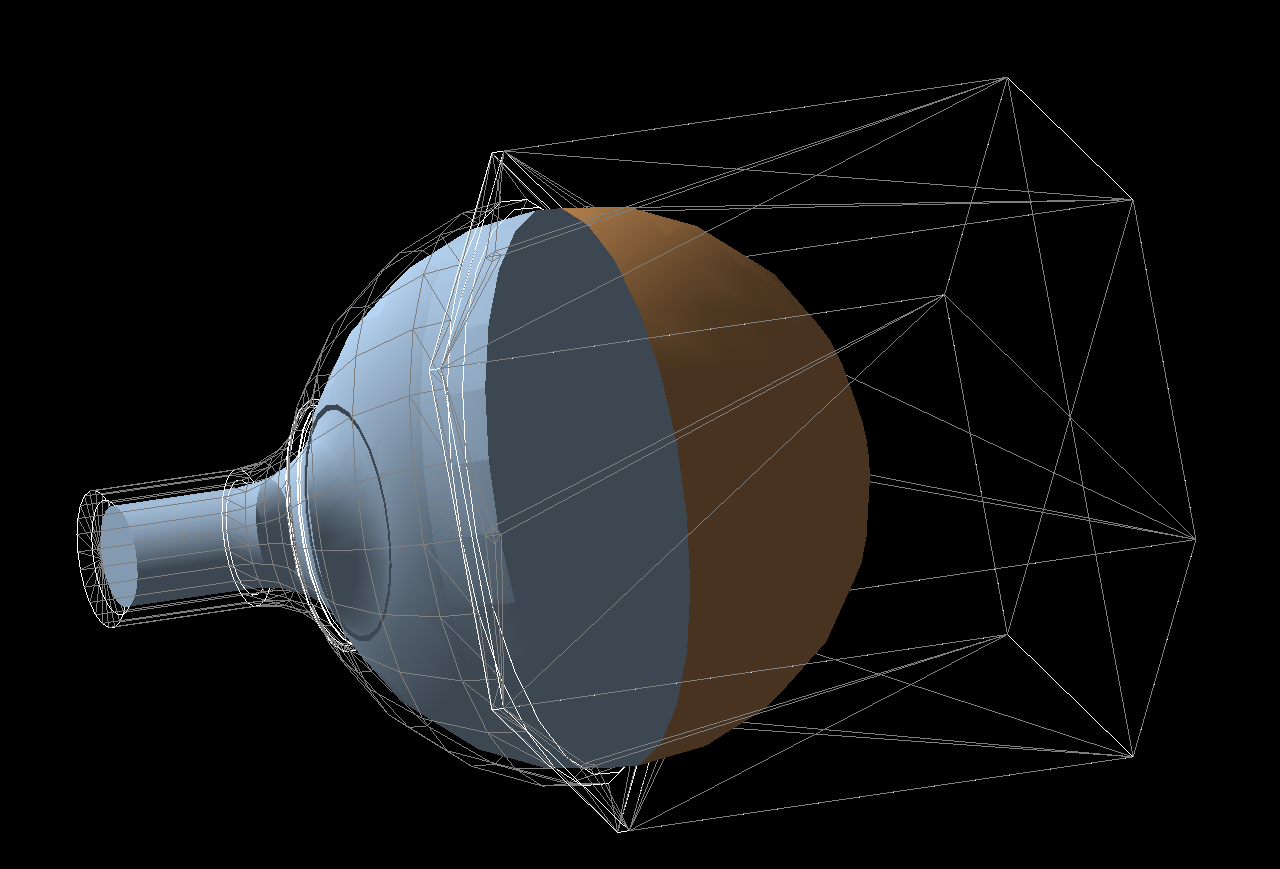
\includegraphics[width=.5\textwidth,keepaspectratio]{data/newpmt-6-sides.png}
        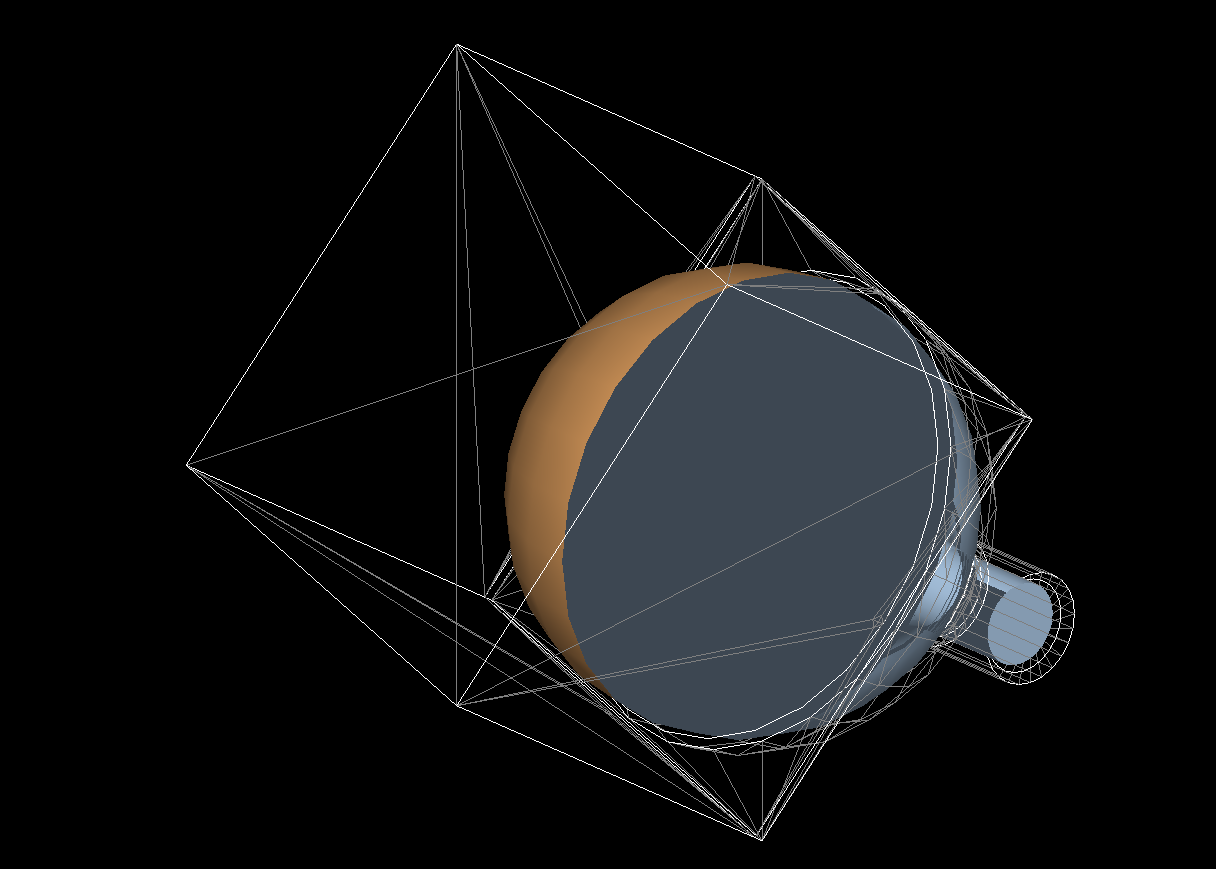
\includegraphics[width=.5\textwidth,keepaspectratio]{data/newpmt-4-sides.png}
    \end{figure}
    在geant4的mac中,使用命令控制PMT/模块
    \begin{itemize}
        \item {\tt /dyb2/det/pmt/type/name HelloPMTCover}使用带外罩的球形PMT
        \item {\tt /dyb2/det/pmt/cover/nside 4}设置外罩的边数
        \item {\tt /dyb2/det/filemode/path
            hexagon.txt}读取文件中设置的位置及旋转
    \end{itemize}
\end{frame}

\begin{frame}
    \frametitle{任意Volume中粒子产生}
    \begin{itemize}
        \item 此处主要需要考虑任意Volume与全局世界之间的仿射变换。
                \footnote{http://en.wikipedia.org/wiki/Affine\_transformation}
        \item 在获取全局与局部的仿射变换后,
              就可以将位置坐标或动量方向
              \footnote{{\tt G4AffineTransform}中已有API可供使用,
                        分别用于点与矢量的变换}
              进行全局与局部之间的转换。
        \item 目前的实现中,需要给定完整的Physical Volume路径,
              根据此路径,计算仿射变换。
        \item 为了避免重复的计算,将路径对应的变换缓存起来。
        \item 例如:{\tt /pWorld/pSteelBall/pTarget}就可以计算pWorld与pTarget
              之间的变换,可用于pTarget中的PMT/模块与pWorld间的变换。
    \end{itemize}
\end{frame}

\subsection{Sniper的开发}

\begin{frame}
    \begin{center}
        \Large Sniper的开发
    \end{center}
\end{frame}

\begin{frame}
    \frametitle{Sniper Python Binding}
    \begin{itemize}
        \item 采用Boost Python库用于Python binding。
        \item binding基本做法
            \begin{itemize}
                \item 用户编写C++代码
                \item 生成对应的库
                \item 以手动/自动的方式编写binding辅助代码
                \item 生成Python可用的库
            \end{itemize}
    \end{itemize}

\begin{tikzpicture}[head/.style={line width=2pt,draw=gray,rounded corners=8pt,text width=2cm,align=center}]
\node[head,fill=green!60!black!50] (wd) {C++源代码};
\node[head,fill=yellow!40,right=of wd] (sa) {对应的动态库};
\node[head,fill=blue!40,right=of sa] (lr) {binding辅助代码};
\node[head,fill=red!40,right=of lr] (rr) {Python可用的库};
\begin{scope}[line width=2pt,gray]
\foreach \box in {wd,sa,lr,rr}
  \draw ([yshift=-5pt]\box.south) -- +(0,-4cm);
\end{scope}
\begin{scope}[every node/.style={single arrow, draw=none,fill=red!50,anchor=west,align=center}]
\node [anchor=west,text width=2.8cm] at ([yshift=-1cm]wd.south) {生成动态库};
\node [anchor=west,text width=6.1cm] at ([yshift=-2cm]wd.south) {生成辅助代码};
\node [anchor=west,text width=2.8cm] at ([yshift=-3cm]lr.south) {链接};
\node [anchor=west,text width=6.1cm] at ([yshift=-3.5cm]sa.south) {链接生成Python可用库};
\end{scope}

\end{tikzpicture}
\end{frame}

\begin{frame}

\end{frame}
